\documentclass[rocket.tex]{subfiles}

\begin{document}

\subsection{Fuerzas y momentos}

Para simulaci�n y desarrollo de c�digo de vuelo se utilizaran los par�metros de referencia indicados en la figura \ref{fig:body-refs}.

En esta se ubican el centro de gravedad CG, el punto de reducci�n para las fuerzas y momentos aerodin�micos, y la ubicaci�n de la articulaci�n del motor.

Las deflexiones del eje de empuje $\delta_y$ y $\delta_z$ se consideran positivas cuando producen aceleraciones angulares tambi�n positivas en la terna del cuerpo.
Esto implica que $\delta_y$ es positiva cuando la tobera del motor apunta hacia arriba ($-z^b$) 
y $\delta_z$ lo es cuando apunta hacia la derecha ($+y^b$).

Con esto la fuerza de empuje resulta:
\begin{equation}
	\vect{T} = 
    \begin{Bmatrix} 
    \phantom{-}	\cos{\delta_y}\cos{\delta_z} \\ 
       -\cos{\delta_y}\sin{\delta_z} \\ 
    	\sin{\delta_y} 
    \end{Bmatrix} 
    \cdot
    T
    \approx
    \begin{Bmatrix} 
    	1 \\ 
       -\sin{\delta_z} \\ 
    \phantom{-}	\sin{\delta_y} 
    \end{Bmatrix} 
    \cdot
    T
\end{equation}
El momento producido por el empuje respecto del CG resulta:
\begin{equation}
	\vect{M}_p = \vect{r}_{gymbal} \times \vect{T}
	\qquad , \qquad
	\vect{r}_{gymbal} = \begin{Bmatrix} x_{cg} - x_{gymbal} \\ 0 \\ 0 \end{Bmatrix}  
\end{equation}
Para c�mputos aerodin�micos es necesario calcular la velocidad relativa del aire en el centro de referencia de los momentos aerodin�micos CA:
\begin{equation}
	\vect{v}_r = \vect{v}^b + \vect{\omega}^b \times \vect{r}_{ca}
	\qquad , \qquad
	\vect{r}_{ca} = \begin{Bmatrix} x_{cg} - x_{ref} \\ 0 \\ 0 \end{Bmatrix}  
\end{equation}
El momento producido por la fuerza aerodin�mica $\vect{F}_a$ en el CG resulta:
\begin{equation}
	\vect{M}_a^b = \vect{M}_a + \vect{r}_{ca} \times \vect{F}_a
\end{equation}

\begin{figure}
	\centering
	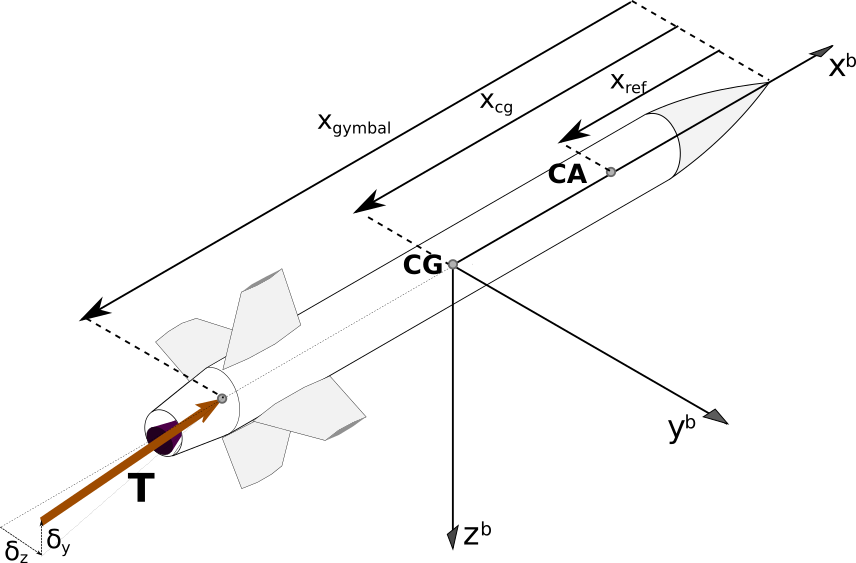
\includegraphics[width=0.75\linewidth]{rocket/body-refs}
	\caption{Par�metros geom�tricos del modelo}
	\label{fig:body-refs}
\end{figure}

\paragraph{Wind axes}

Las fuerzas aerodin�micas pueden obtenerse con coeficientes en terna del cuerpo ($\{X^b, Y^b, Z^b\}$) o terna de viento ($\{D, Y, L\}$). 
Para interpolar resulta mejor esto �ltimo, pero el resultado debe proyectarse en terna-$b$ teniendo en cuenta loas �ngulos de ataque y deslizameinto: 
\begin{equation*}
	\vect{f}^b = \mtx{C}_\alpha \mtx{C}_\beta \begin{bmatrix} -D \\ \phantom{-}Y \\ -L \end{bmatrix}
\end{equation*}
donde:
\begin{equation*}
	\mtx{C}_\alpha 	= \begin{bmatrix} \cos\alpha & 0 & -\sin\alpha \\ 0 & 1 & 0 \\ \sin\alpha & 0 & \phantom{-}\cos\alpha \end{bmatrix}
	\qquad , \qquad 
	\mtx{C}_\beta	= \begin{bmatrix} \phantom{-}\cos\beta & \sin\beta & 0 \\ -\sin\beta & \cos\beta & 0 \\ 0 & 0 & 1 \end{bmatrix}
\end{equation*}
Teniendo en cuenta los signos de las fuerzas:
\begin{equation}
	\mtx{C}^b_w =
	\begin{bmatrix} 
	-\cos\alpha\cos\beta & \cos\alpha\sin\beta &  \sin\alpha \\ 
	 \sin\beta           & \cos\beta           &  0 \\ 
	-\cos\beta\sin\alpha & \sin\alpha\sin\beta & -\cos\alpha 
	\end{bmatrix}
\end{equation}
 


\subsection{Navegaci�n}

Para la cinem�tica del veh�culo un modelo en coordenadas ECEF: 
\begin{align*}
	\dot{\vect{p}}^e   &= \vect{v}^e  \\
	\dot{\vect{v}}^e   &= \mtx{C}_b^e\vect{f}^b + \vect{\gamma}^e\left(\vect{p}^e\right) - 2\mathbf{\Omega}_{ie}^e\times\vect{v}^e \\
	\dot{\vect{q}}_b^e &= \frac{1}{2}\vect{q}_b^e \begin{Bmatrix} \vect{\omega}_{eb}^b \\ 0 \end{Bmatrix}
                      	 -\frac{1}{2}\begin{Bmatrix} \vect{\Omega}_{ie}^e\\0 \end{Bmatrix}\vect{q}_b^e
                      	 \\ \\
    \vect{f}^b &= 
    \frac{1}{m}
    \begin{Bmatrix} 
    	X(\sigma, \alpha, \beta, \mathcal{M}) + T \\ 
    	Y(\sigma, \alpha, \mathcal{M}) - T \sin \delta_z \\ 
    	Z(\sigma, \beta , \mathcal{M}) + T \sin \delta_y 
    \end{Bmatrix} 
    +
    \frac{1}{m}
    \begin{Bmatrix} 
    	0 \\ 
    	Y_{\dot{\beta }} \dot{\beta } \\ 
    	Z_{\dot{\alpha}} \dot{\alpha}
    \end{Bmatrix}     
    - \dot{m} \vect{v}             	 
\end{align*}

Para los �ngulos de incidencia se propone:
\begin{align*} 
	\alpha &= \tan^{-1} \frac{w^b}{u^b} \approx \frac{w^b}{V} \\
	\beta  &= \sin^{-1} \frac{v^b}{V}   \approx \frac{v^b}{V} \\
	\dot{\alpha} &= \frac{1}{u^2 + w^2} \left(u \dot{w} - w \dot{u}\right)  
\end{align*}



%Utilizamos la ecuaci�n \eqref{ecu:tray_v_dot} para los cambios en la velocidad, pero para la senda de ascenso $\gamma$ debemos agregar la la fuerza normal a la \eqref{ecu:tray_gamma_dot} cuando $\alpha \neq 0$.
%Para el �ngulo de ataque se tiene que:
%\begin{equation*} 
%	\alpha = \sin^{-1} \frac{w^b}{V} \approx \frac{w^b}{V}
%\end{equation*}
%y para el �ngulo de la velocidad:
%\begin{equation*} 
%	\gamma = \theta - \alpha 
%\end{equation*}
%con lo cual
%\begin{equation*} 
%	\dot{\gamma} = \dot{\theta} - \dot{\alpha} 
%	%           \\&= q - \frac{\partial \alpha}{\partial w} \dot{w} - \frac{\partial \alpha}{\partial V}\dot{V}
%	           = q - \frac{1}{V} \dot{w} + \frac{w}{V^2}\dot{V}
%\end{equation*}
%Y como $w = V \sin \theta$:
%\begin{equation*} 
%	\dot{\gamma} = q - \frac{1}{V} \left(\dot{w} - \dot{V} \sin \theta \right)
%\end{equation*}
%De la suma de fuerzas en $z^b$ tenemos que:
%\begin{equation*} 
%	\dot{w} = g \cos \theta - f_N \sin \alpha
%\end{equation*}
%con lo cual finalmente:
%\begin{equation*} 
%	\dot{\gamma} = q - \frac{1}{V} \left(g \cos \theta - f_N \sin \alpha - \dot{V} \sin \theta \right)
%\end{equation*}


%donde $w$ es la componente vertical de la velocidad (con eje $z^e$ apuntando hacia abajo)

\end{document}
